Machine learning has become an extremely powerful tool in the realm of computer vision, particularly through the use of convolutional neural networks (CNNs) and the increased availability of data and computational resources. This chapter introduces the fundamentals of CNNs, as well as their application to computer vision and robotics.

\notessection{Modern Computer Vision}
Modern computer vision techniques\cite{ForsythPonce2011} rely heavily on deep learning and convolutional neural network architectures\cite{GoodfellowBengioEtAl2016}. A convolutional neural network is a type of neural network with additional structure that is beneficial for image processing tasks. In fact, CNNs can be said to be ``regularized'' neural networks since the additional structure reduces the ability of the network to overfit to data.
This chapter will introduce each component\footnote{Convolutional layers, nonlinear activations, pooling layers, and fully-connected layers.} in the architecture of a CNN, and then discuss how CNNs can be applied to problems in robotics.

\begin{figure}[ht] 
\begin{center}
\includegraphics[width=\textwidth]{tex/figs/ch12_figs/lecun.png}
\caption{Example convolutional neural network architecture from LeCun et al. (1998)\nocite{LecunBottouEtAl1998}.}
\label{fig:activations}
\end{center}
\end{figure}

\subsection{Convolutional Neural Networks}

\subsubsection{Convolution Layers}
\begin{marginfigure} 
\begin{center}
\includegraphics[width=0.75\textwidth]{tex/figs/ch12_figs/convolution.png}
\caption{A convolution filter being applied to a 3-channel RGB image.}
\label{fig:convfilter}
\end{center}
\end{marginfigure}
One of the main structural concepts that is unique to the architecture of a CNN is the use of convolution layers. 
These layers exploit the underlying \textit{spatial locality} structure in images by using sliding ``learned'' filters, which are often much smaller than the image itself. Mathematically these filters perform operations in a similar way as other linear filters that have been used in image processing, such as Gaussian smoothing filters, and can be expressed as affine functions:
\begin{equation*}
    f(x) = w^\top x + b,
\end{equation*}
where $w$ is a vectorized representation of the weight parameters that define the filter, $x$ is a vectorized version of the image pixels covered by the filter, and $b$ is a scalar bias term.
For example in Figure \ref{fig:convfilter} a filter is applied over an image with three color channels (red, green, blue). In this case the filter may have dimension $m \times n \times 3$, which could be vectorized to a weight vector $w$ with $3mn$ elements. Additionally, the \textit{stride} of the filter describes how many positions it shifts by when sliding over the input. The output of the filter is also passed through a nonlinear activation, typically a ReLU function.

Once the filter has been applied to the entire image, the collection of outputs from the activation function will create a new ``filtered image'' typically referred to as an \textit{activation map.}
\begin{figure}[ht] 
\begin{center}
\includegraphics[width=0.45\textwidth]{tex/figs/ch12_figs/convolution2.png}
\caption{The outputs of a convolution filter and activation function applied across an image make up a new image, called an \textit{activation} map.}
\label{fig:activations}
\end{center}
\end{figure}
In practice a number of different filters are usually learned in each convolution layer, which would simply produce a corresponding number of activation maps as the output\footnote{Besides the number of filters applied to the input, the width and height of the filter, the amount of padding on the input, and the stride of the filter are other hyperparameters.}. This is crucial such that each filter can focus on learning one specific relevant feature. Examples of different filters that might be learned in different convolution layers of a CNN are shown in Figure \ref{fig:convfeatures}\cite{ZeilerFergus2014}. Notice that the low-level features which are learned in earlier convolution layers look a lot like edge detectors (i.e. are more basic/fundamental) while later convolution layers have filters that look more like actual objects.
\begin{figure}[ht] 
\begin{center}
\includegraphics[width=0.65\textwidth]{tex/figs/ch12_figs/features.png}
\caption{Low-level, mid-level, and high-level feature visualizations in a convolutional neural network from Zeiler and Fergus (2014)\nocite{ZeilerFergus2014}.}
\label{fig:convfeatures}
\end{center}
\end{figure}

In general, the use of convolution layers to exploit the spatial locality of images provides several benefits including:
\begin{enumerate}
    \item \textit{Parameter sharing}: the (small) filter's parameters are applied at all points on the image. Therefore the total number of learned parameters in the model is much smaller than if a fully-connected layer was used.
    \item \textit{Sparse interactions}: having the filter be smaller than the image allows for better detection of smaller, more meaningful features and improves computation time by requiring fewer mathematical operations to evaluate.
    \item \textit{Equivariant representation:} the convolution layer is equivariant to translation, meaning that the convolution of a shifted image is equivalent to the shifted convolution of the original image\footnote{However, convolution is not equivariant to changes in scale or rotation.}.
    \item The ability to work with images of \textit{varying size} if needed.
\end{enumerate}


\subsubsection{Pooling Layers}
Pooling is the second major structural component in CNNs. Pooling layers typically come after convolution layers (and their nonlinear activation functions). Their primary function is to replace the output of the convolution layer's activation map at particular locations with a ``summary statistic'' from other spatially local outputs. This helps make the network more robust against small translations in the input, helps improve computational efficiency by reducing the size of the input (i.e. it lowers the resolution), and is useful in enabling the input images to vary in size\footnote[][-2\baselineskip]{The size of the pooling can be modified to keep the size of the pooling layer output constant.}. The most common type of pooling is \textit{max} pooling, but other types also exist (such as \textit{mean} pooling). 

\begin{marginfigure} 
\begin{center}
\includegraphics[width=0.95\textwidth]{tex/figs/ch12_figs/maxpool.png}
\caption{Max pooling example with $2 \times 2$ filter and stride of $2$.}
\label{fig:pooling}
\end{center}
\end{marginfigure}
Computationally, both max and mean pooling layers operate with the same filtering idea as in the convolution layers. Specifically, a filter of width $m$ and height $n$ slides around the layer's input with a particular stride. The difference between the two comes from the mathematical operation performed by the filter, which as their names suggest are either a maximum element or the mean over the filter. If the output of the convolution layer has $N$ activation maps, the output of the pooling layer will also have $N$ ``images'', since the pooling filter is only applied across the spatial dimensions.

\subsubsection{Fully Connected Layers}
Downstream of the convolution and pooling layers are fully connected layers. These layers make up what is essentially just a standard neural network, which is appended to the end of the network. The function of these layers is to take the output of the convolution and pooling layers (which can be thought of as a highly condensed representation of the image) and actually perform a classification or regression. Generally the total number of fully connected layers at the end of the CNN will only make up a fraction of the total number of layers.

\subsubsection{CNN Performance}
A CNN can be said to learn how to process images \textit{end-to-end} because it essentially learns how to perform two steps simultaneously: feature extraction and classification or regression (i.e. it learns the entire process from image input to the desired output). In contrast, classical approaches to image processing use hand-engineered feature extractors. Since 2012, the performance of end-to-end learning approaches to image processing have dominated and continue to improve\footnote{Of course in some specific applications hand-engineered features may still be better! For example if engineering insight can identify a structure to the problem that a CNN could not.}. This continuous improvement has generally been realized with the use of deeper networks.

\subsection{CNNs for Object Detection and Localization}
Modern computer vision techniques such as convolutional neural networks have a large variety of applications in robotic perception, including object localization and detection.

In object localization problems, the goal is to identify the position of an object in the image. This is usually accomplished by specifying four numbers that define a \textit{bounding box} for the object in the image\footnote{Box coordinates are usually the $(x,y)$ position of the top-left corner and the width $w$ and height $h$ of the box.} (see Figure \ref{fig:boundingbox}). To solve object localization problems with a CNN, the standard approach is to have the output of the network be both the bounding box coordinates and an object class. This can be accomplished by reusing the convolution and pooling layers of the CNN but then have two separate branches of the fully connected layers: one trained for classification and the other for localization\footnote{Since the output of the localization branch is four real numbers $(x,y,w,h)$, this would be considered a regression problem and it is common to use and $l_2$ loss function.}. To train a network to simultaneously perform classification and localization, a multi-task loss function can be defined by adding together the loss functions of each branch.
\begin{figure}[ht] 
\begin{center}
\includegraphics[width=0.5\textwidth]{tex/figs/ch12_figs/boundingbox.png}
\caption{Bounding box prediction for several objects in an image from Ren, He, et al. (2017)\nocite{RenHeEtAl2017}}
\label{fig:boundingbox}
\end{center}
\end{figure}

If multiple objects exist within a single image the object localization and classification problem becomes more difficult. First, the number of outputs of the network may change! For example, outputting a bounding box for $n$ objects would require $4n$ outputs. A practical solution to handling the problem of varying outputs is to simply apply the CNN to a series of cropped images produced from the original image, where the network can also classify the image as ``background'' (i.e. not an object)\footnote{This could be thought of as applying the entire CNN as a filter that slides across the image.}. 
However, a naive implementation of this idea would likely result in an excessive number of CNN evaluations. Instead, different approaches have been developed for making this idea efficient by reducing the number of areas in the image that need to be evaluated. For example this has been accomplished by identifying ``regions of interest'' in the image through some other approach, or even partitioning the image into a grid.
